% 2021-09-01 by Banbara
\documentclass[dvipdfmx,11pt]{beamer}

%%% Package
% \usepackage{bxdpx-beamer}
% \usepackage{pxjahyper}
% \usepackage{minijs}
% \usepackage{otf}
% \renewcommand{\kanjifamilydefault}{\gtdefault}

%%% My Macro
\usepackage{ipsj}
\usepackage{color}
\usepackage{amssymb}
\usepackage{amsmath}
\usepackage{amsthm}
\usepackage{multirow,bigdelim}
\newcommand{\la}{\leftarrow}
\newcommand{\Lra}{\Longrightarrow}
\newcommand{\Lla}{\Longleftarrow}
\newcommand{\Llra}{\Longleftrightarrow}
\newcommand{\lra}{\longrightarrow}
\newcommand{\dd}{\mathop{..}}
\newcommand{\range}[2]{\{#1\dd#2\}}
\newcommand{\imp}{\Rightarrow}
\newcommand{\equ}{\Leftrightarrow}
\renewcommand{\labelenumi}{(\arabic{enumi})}
\newcommand{\alldiff}{\textrm{alldifferent}}
\newcommand{\Alldiff}{\alldiff(x_1,x_2,\ldots,x_n)}
\newcommand{\SAT}{{\tt SAT}}
\newcommand{\UNSAT}{{\tt UNSAT}}
\newcommand{\Dom}{{\it Dom}}
% \newcommand{\p}[2]{p(#1,#2)}
\newcommand{\dE}[2]{p(#1=#2)}
\newcommand{\lE}[2]{p(#1^{(#2)})}
\newcommand{\oE}[2]{p(#1\le#2)}


%%% Beamer
% \usetheme{Copenhagen}
% \usetheme{Warsaw}
\usetheme{Madrid}
\usefonttheme{structurebold}
% \usefonttheme{professionalfonts}
% \setbeamertemplate{blocks}[shadow=true,rounded]
% \setbeamercolor{structure}{fg=blue!50!black}
% \setbeamercolor{alerted text}{fg=red!70!black}
% \setbeamercolor{item projected}{fg=black,bg=blue!20!white}
\setbeamertemplate{navigation symbols}{}
% \useoutertheme[subsection=false]{miniframes}
\setbeamertemplate{footline}[frame number]
% exclude apprendix slides from framenumber
\newcommand{\backupbegin}{
  \newcounter{framenumberappendix}
  \setcounter{framenumberappendix}{\value{framenumber}}
}
\newcommand{\backupend}{
  \addtocounter{framenumberappendix}{-\value{framenumber}}
  \addtocounter{framenumber}{\value{framenumberappendix}} 
}

%%% Title page
\title{解集合プログラミングを用いた組合せ遷移ソルバーに関する研究}
\author{山田 悠也}
\date{2022年2月16日\\前期課程中間発表会}
\institute{番原研究室}

%%%%%%%%%%%%%%%%%%%%%%%%%%%%%%%%%%%%%%%%%%%%%%%%%%%%%%%%%%%%%%%%%
\begin{document}
\maketitle
%%%%%%%%%%%%%%%%%%%%%%%%%%%%%%%%%%%%%%%%%%%%%%%%%%%%%%%%%%%%%%%%%
\begin{frame}
  \frametitle{組合せ遷移 (Combinatorial Reconfiguration)}
  \begin{alertblock}{組合せ遷移問題とは}
    基となる組合せ問題とその2つの実行可能解が与えられたとき,
    一方の実行可能解から他方の実行可能解へ,遷移制約を満たしつつ,
    実行可能解のみを経由して到達できるかを判定する問題
  \end{alertblock}

  \begin{itemize}
  \item 近年,理論計算機科学の分野を中心に急速に発展し,理論的な基盤が
    整備されつつある\footnotemark[1].
  \item 基となる問題が NP 完全であるとき,その遷移問題の多くは
    \alert{\bf PSPACE完全}であることが知られている.
    \begin{itemize}
%    \item 命題論理の充足可能性判定(SAT)の遷移問題~[Gopalan+,'09]
    \item 独立点集合の遷移問題~[Ito+,'11]
%    \item 集合被覆の遷移問題~[Ito+,'11]
    \item \structure{グラフ点彩色の遷移問題}~[Bonsma+,'09]
%    \item 15パズル
    \end{itemize}
  \item 工学的にも,配電網の切替えなど持続的システムへの実用的応用が期
    待されている.
  \item 競技会も開催され,実践面でも研究が発展することが予想される.
  \end{itemize}

  \begin{alertblock}<2>{}\centering
    しかしながら,現状では,組合せ遷移問題を解く
    \alert{\bf 汎用ソルバーの実装技術は確立されていない}.
  \end{alertblock}

  \footnotetext[1]{Web Portal: http://www.ecei.tohoku.ac.jp/alg/core/}
\end{frame}
%%%%%%%%%%%%%%%%%%%%%%%%%%%%%%%%%%%%%%%%%%%%%%%%%%%%%%%%%%%%%%%%%
\begin{frame}
  \frametitle{グラフ点彩色問題を基とする遷移問題}
  \begin{exampleblock}{色数$k=3$のグラフ点彩色問題}\centering
    \begin{tabular}[t]{ccc}
      \scalebox{0.55}{グラフ名 & 頂点数 & 辺数 & 要素数$k$ & 解の総数 \\ \hline
\code{grid004x004} & 16 & 24 & 6 & 114 \\
\code{grid004x004} & 16 & 24 & 7 & 20 \\
\code{hc-power-11} & 21 & 28 & 9 & 32 \\
\code{hc-power-12} & 36 & 51 & 15 & 256 \\
\code{hc-square-01} & 14 & 18 & 6 & 15 \\
\code{hc-square-02} & 24 & 33 & 10 & 75 \\
\code{hc-toyno-01} & 6 & 9 & 2 & 6 \\
\code{hc-toyyes-01} & 7 & 7 & 3 & 8 \\\hline

}
      &
      \rz{$\Rightarrow$}
      &
      \scalebox{0.55}{\input{graph_colored}}
    \end{tabular}
  \end{exampleblock}
  \pause
  \begin{block}{$k$彩色遷移問題}
    \begin{itemize}
    \item \structure{\bf 入力}:
      色数$k$のグラフ点彩色問題と,スタート状態とゴール状態
      を表す2つの実行可能解
    \item \structure{遷移制約}: 1回の遷移で色が変化する頂点はただ1つのみ
    \item \structure{目的}:
      スタート状態からゴール状態への到達可能性を判定
    \end{itemize}
  \end{block}
  \begin{itemize}
  \item 代表的な組合せ遷移問題の一つである.
  \item 一般に$k \geq 4$で PSPACE 完全であることが知られている.
  \end{itemize}

\end{frame}
%%%%%%%%%%%%%%%%%%%%%%%%%%%%%%%%%%%%%%%%%%%%%%%%%%%%%%%%%%%%%%%%%
\begin{frame}%[shrink]
  \frametitle{$k=4$彩色遷移問題の例}
  \begin{center}
  \tabcolsep = 3mm
  \renewcommand{\arraystretch}{1.2}
  \begin{tabular}[t]{ccc}
    スタート状態($t=0$) && \uncover<2>{$t=1$} \\
    \scalebox{0.5}{\input{gcrp_t0}} &
    \uncover<2>{\rz{\Large$\Rightarrow$}} &
    \uncover<2>{\scalebox{0.5}{\input{gcrp_t1}}}\\
    && \uncover<2>{\Large $\Downarrow$} \\
    \scalebox{0.5}{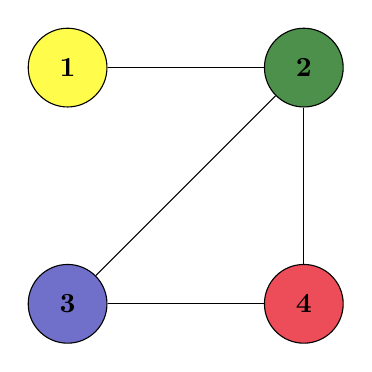
\begin{tikzpicture}[x=1.5cm, y=1.5cm]
  % 設定
  \tikzset{node/.style={circle,draw=black,minimum size=1cm}}
 
  %色
  \definecolor{red}{RGB}{230,0,18}
  \definecolor{blue}{RGB}{51,51,179}
  \definecolor{yellow}{RGB}{255,251,0}
  \definecolor{green}{RGB}{0,96,0}
 
  % 補助線
  % \draw [help lines,blue] (0,0) grid (20,6);
 
  % node %
  \node[node, fill=yellow!70] at (-1,1) (node1) {\textbf{1}};
  \node[node, fill=green!70] at (1,1) (node2) {\textbf{2}};
  \node[node, fill=blue!70] at (-1,-1) (node3) {\textbf{3}};
  \node[node, fill=red!70] at (1,-1) (node4) {\textbf{4}};
 
  \foreach \u / \v in {node1/node2, node2/node3, node2/node4, node3/node4}
  \draw (\u) -- (\v);
\end{tikzpicture}
} &
    \uncover<2>{\rz{\Large$\Leftarrow$}} &
    \uncover<2>{\scalebox{0.5}{\input{gcrp_t2}}}\\
    ゴール状態\uncover<2>{($t=3$)} && \uncover<2>{$t=2$}
  \end{tabular}
  \end{center}

  \uncover<2>{
  \begin{itemize}
  \item スタート状態からゴール状態へ3ステップで到達可能である.
  \item 各ステップ$t$において,グラフ点彩色問題の制約を満たす.
  \item 1回の遷移において,色が変化する頂点はただ1つのみである.
  \end{itemize}
  }
\end{frame}
%%%%%%%%%%%%%%%%%%%%%%%%%%%%%%%%%%%%%%%%%%%%%%%%%%%%%%%%%%%%%%%%%
\begin{frame}
  \frametitle{解集合プログラミング {\large(Answer Set Programming; ASP)}}
  \begin{itemize}
  \item \structure{ASP 言語}は,一階論理に基づく知識表現言語の一種.
  \item \structure{ASP システム}は,論理プログラムから
    安定モデル意味論~{\scriptsize[Gelfond and Lifschitz, '88]}
    に基づく解集合を計算するシステム.
  \item 近年,SAT 技術を応用した高速 ASP システムが開発され,
    システム生物学,プランニング,モデル検査など様々な分野への実用的応
    用が急速に拡大している.
  \end{itemize}

  \begin{alertblock}{組合せ遷移問題に対してASPを用いる利点}
    \begin{itemize}
    \item ASPの高い表現力により,様々な組合せ問題を簡潔に記述できる.
      \begin{itemize}
      \item \alert{\bf 遷移問題への拡張も容易}.
      \end{itemize}
    \item インクリメンタルASP解法により,ステップ長を増やしながら,
      遷移問題の\alert{\bf 到達可能性を効率的に検査}できる.
      \begin{itemize}
      \item ASP システムを複数回起動するオーバーヘッドを回避.
      \item 同様の探索失敗を避けるために獲得した学習節を再利用.
      \end{itemize}
    \item 探索ヒューリスティックスを簡単にカスタマイズできる.
    % \item ASP Modulo Theories 技術により,様々な背景理論ソルバーと連携が可能である.
    \end{itemize}
  \end{alertblock}
\end{frame}
%%%%%%%%%%%%%%%%%%%%%%%%%%%%%%%%%%%%%%%%%%%%%%%%%%%%%%%%%%%%%%%%% 
\begin{frame}
  \frametitle{研究目的}
  \begin{alertblock}{研究目的}
    ASP 技術を活用し,組合せ遷移問題を効率よく解くソルバーを実現する.
  \end{alertblock}
  \begin{itemize}
  \item 方針: プランニングや有界モデル検査のための技法を応用
  \end{itemize}

  \begin{block}{卒業研究の内容}
    \begin{itemize}
      \item 組合せ遷移問題に対してステップ長$\ell$を導入し解く手法に基づき,
        $k$彩色遷移問題の3つの符号化を考案・評価.
    \end{itemize}
  \end{block}

  \begin{block}{その後の研究内容}
    \begin{itemize}
      \item ステップ長$\ell$を導入して解く手法を
        \alert{有界組合せ遷移}として定式化.
 %     \item インクリメンタル ASP 解法を利用し,基本ソルバーの
 %       問題点を改良した改良ソルバーを考案・評価.
      \item ソルバーを構成する2つのアルゴリズムの考案.
        \begin{itemize}
          \item \structure{基本アルゴリズム}
          \item \structure{改良アルゴリズム}
        \end{itemize}
      \item 各アルゴリズムを実装した2つのソルバーの評価.
      \item 独立点集合の遷移問題を解く ASP 符号化の考案.
    \end{itemize}
  \end{block}
\end{frame}
%%%%%%%%%%%%%%%%%%%%%%%%%%%%%%%%%%%%%%%%%%%%%%%%%%%%%%%%%%%%%%%%%%%
\begin{frame}{ASP 技術を用いた組合せ遷移ソルバーの実装}

\begin{alertblock}{}\centering
開発した組合せ遷移ソルバーの構成図は以下の通りである.
\end{alertblock}
\vfill
\begin{center}
\setlength{\unitlength}{1.0pt}
\scriptsize\tiny
\thicklines
%  \begin{figure*}[t]
  \centering
  \thicklines
  \setlength{\unitlength}{1.28pt}
  \small
  \begin{picture}(280,57)(4,-10)
    \put( -35, 20){\dashbox(70,24){\shortstack{組合せ最適化問題\\のインスタンス}}}
    \put( 45, 20){\framebox(50,24){変換器}}
    \put(105, 20){\dashbox(70,24){\shortstack{ASPファクト}}}
    \put(105,-10){\dashbox(70,24){\shortstack{ASP符号化\\(論理プログラム)}}}
    \put(185,-10){\framebox(60,54){}}
    \put(189, 25){\framebox(52,12){ASPソルバー}}
    \put(190, -5){\framebox(50,12){LNPS}}
    % \put(180, 20){\framebox(50,24){ASPシステム}}
    \put(255, 20){\dashbox(70,24){\shortstack{組合せ最適化問題\\の最適解}}}
    \put(  35, 32){\vector(1,0){10}}
    \put(  95, 32){\vector(1,0){10}}
    \put(175, 32){\vector(1,0){10}}
    \put(245, 32){\vector(1,0){10}}
    \put(175, +2){\line(1,0){4}}
    \put(179, +2){\line(0,1){30}}
    \put(205,  7){\vector(0,1){17}}
    \put(225, 24){\vector(0,-1){17}}
    \put(190, 48){提案ソルバー}
  \end{picture}  
\caption{提案ソルバー\textit{asprior}の構成}
\label{fig:arch}
\end{figure*}

%%% Local Variables: 
%%% mode: latex
%%% TeX-master: "paper"
%%% End: 

\begin{picture}(280,57)(4,-10)
  \put(  0, 20){\dashbox(50,24){\shortstack{組合せ遷移問題\\のインスタンス}}}
  \put( 60, 20){\framebox(50,24){変換器}}
  \put(120, 20){\dashbox(50,24){\shortstack{ASPファクト}}}
  \put(120,-10){\dashbox(50,24){\shortstack{論理プログラム\\(ASP符号化)}}}
  \put(180,-10){\alert{\framebox(50,54){}}}
  \put(185, 27){\framebox(40,12){ASP システム}}
  \put(185, -5){\alert{\bf\framebox(40,18){\shortstack{有界組合せ遷移\\アルゴリズム}}}}
  \put(240, 20){\dashbox(50,24){\shortstack{組合せ遷移問題\\の解}}}
  \put( 50, 32){\vector(1,0){10}}
  \put(110, 32){\vector(1,0){10}}
  \put(170, 32){\vector(1,0){10}}
  \put(230, 32){\vector(1,0){10}}
  \put(170, +2){\line(1,0){4}}
  \put(174, +2){\line(0,1){30}}
  \put(195, 13){\vector(0,1){14}}
  \put(215, 27){\vector(0,-1){14}}
  \put(188, 50){\alert{\bf 提案ソルバー}}
\end{picture}  
\end{center}
  
\begin{enumerate}
\item 問題インスタンスを ASP のファクト形式に変換する.
\item ASP ファクトと組合せ遷移問題を解く
  論理プログラム(ASP符号化)を入力として,
  \alert{\bf 提案ソルバー}を用いて解集合を計算する.
\item 解集合を解釈して,組合せ遷移問題の解を得る.
\end{enumerate}
\begin{alertblock}{}
  有界組合せ遷移のためのアルゴリズムとして,
  基本アルゴリズムと改良アルゴリズムの2種類を考案した.
\end{alertblock}
\end{frame}
%%%%%%%%%%%%%%%%%%%%%%%%%%%%%%%%%%%%%%%%%%%%%%%%%%%%%%%%%%%%%%%%%%%
\begin{frame}\frametitle{実験概要}
  \begin{block}{}\centering
    提案したソルバーの有効性を評価するにあたり,以下の実験を行った.
  \end{block}
  \bigskip
  \begin{itemize}
  \item \structure{比較に用いたソルバー}
    \begin{itemize}
    \item 基本ソルバー$\cdots$基本アルゴリズムを実装
    \item 改良ソルバー$\cdots$改良アルゴリズムを実装
    \end{itemize}
  \item \structure{比較に用いたASP符号化}
    \begin{itemize}
    \item \code{changed}符号化
    \item \code{unchanged}符号化
    \end{itemize}
  \item \structure{ベンチマーク問題}: \alert{\bf 独自に作成した$k$彩色遷移問題(計90問)}
    \begin{itemize}
    \item \textit{COLOR04}で公開されているグラフ点彩色問題のグラフ127個のうち,
      彩色数が判明している44個~[Tamura+,'09] を候補とした.
    \item 最終的に,彩色数での実行可能解を全列挙することができたグラフ9個を使用した.
    \end{itemize}
  % \item \structure{ステップ長の上限値}: 基となるグラフ点彩色問題の実行
  %   可能解の総数から1引いた数
    % \begin{itemize}
    % \item グラフmyciel4から作成した問題については,{\clingo}が対応している数
    %   よりも解の総数が大きかったため,
    %   上限値を$2^{31}-1$とした.
    % \end{itemize}
    \item \structure{ASPシステム}: \textit{clingo-5.4.0} \textit{jumpy}
    \item \structure{制限時間}: 3600秒/問
    \item \structure{環境}: Mac OS, 3.2GHz 6コア Intel Core i7,64GB メモリ
    \end{itemize}
\end{frame}
%%%%%%%%%%%%%%%%%%%%%%%%%%%%%%%%%%%%%%%%%%%%%%%%%%%%%%%%%%%%%%%%%%%
\begin{frame}\frametitle{実験結果: 解けた問題数}

  \begin{exampleblock}{}
    \centering
    \renewcommand{\arraystretch}{1.2}
    \scalebox{0.9}{\begin{tabular}{l|rrr} 
  & 到達可能 & 到達不能 & 合計 \\ \hline
  origin & 11 & 0 & 11 \\
  changed & 11 & 10 & 21 \\
  unchanged & 11 & 10 & 21 \\
\end{tabular}}
  \end{exampleblock}

  \begin{itemize}
  \item 90問中71問について,到達可能性を判定できた.
    \begin{itemize}
    \item 到達可能11問,到達不能60問
    \end{itemize}
  \item 改良ソルバーと\code{unchanged}符号化の組合せが,
    最も多くの問題を解いた.平均CPU時間も最も短い.
%  \item 到達可能であることが判定できた問題のうち,最長のステップ長は17であった.
  \item 到達不能なインスタンスについて,インクリメンタル解法を用いた改
    良ソルバーの優位性が確認できた.
  \end{itemize}
\end{frame}
%%%%%%%%%%%%%%%%%%%%%%%%%%%%%%%%%%%%%%%%%%%%%%%%%%%%%%%%%%%%%%%%%%% 
\begin{frame}\frametitle{実験結果: カクタスプロット}

  \begin{figure}[h]
    \centering
    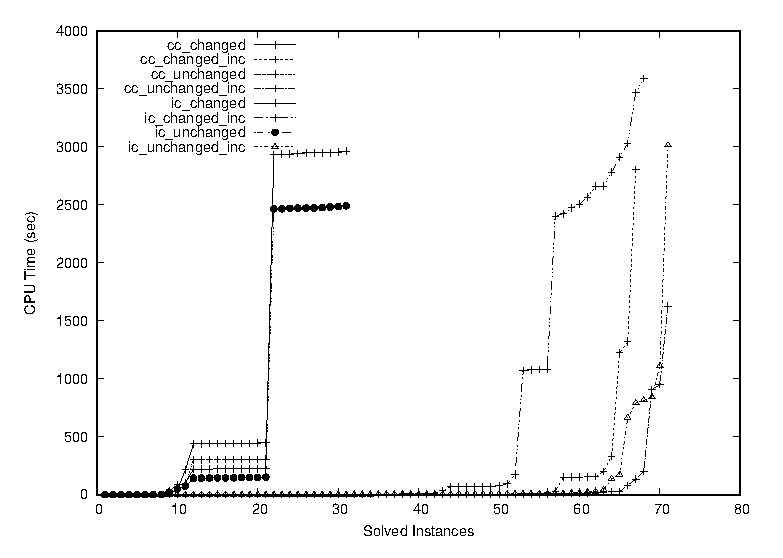
\includegraphics[scale=0.7]{fig/cactus.eps}
  \end{figure}

  \begin{itemize}
    \item 改良ソルバーは基本ソルバーより多くの問題を高速に解いている.
    \item \code{unchanged} 符号化は,\code{changed}符号化より良い性能
      を示した.
  \end{itemize}
  
\end{frame}
%%%%%%%%%%%%%%%%%%%%%%%%%%%%%%%%%%%%%%%%%%%%%%%%%%%%%%%%%%%%%%%%%%%
\begin{frame}\frametitle{まとめ}

  \begin{alertblock}{本研究の成果}\centering
    ASP を用いた組合せ遷移問題の解法として有界組合せ遷移を提案し,
    汎用ソルバーの実装および$k$彩色遷移問題を用いた性能評価を行なった.
  \end{alertblock}

  \begin{enumerate}
  \item \structure{2種類の実装方式の考案}
    \begin{itemize}
    \item 基本アルゴリズム
    \item インクリメンタルASP解法を用いた改良アルゴリズム
    \end{itemize}
  \item \structure{$k$彩色遷移問題を解く2種類の ASP 符号化の考案}
  \item \structure{$k$彩色遷移問題のベンチマーク問題を独自に生成}
  \item \structure{$k$彩色遷移問題を用いた有界組合せ遷移の評価実験}
    \begin{itemize}
    \item 改良アルゴリズムの優位性を確認
    \end{itemize}
  \end{enumerate}
  
  \begin{exampleblock}{今後の課題}
    \begin{itemize}
      \item 組合せ遷移問題の記述例の蓄積
        \begin{itemize}
          \item 現在,競技会のベンチマークでもある,
            \structure{独立点集合の遷移問題}を対象として取組んでいる.
        \end{itemize}
      \item ソルバーの高速化
    \end{itemize}
  \end{exampleblock}
\end{frame}
%%%%%%%%%%%%%%%%%%%%%%%%%%%%%%%%%%%%%%%%%%%%%%%%%%%%%%%%%%%%%%%%%%%
\begin{frame}\frametitle{研究業績}
  \begin{itemize}
    \item \structure{受賞}
    \begin{itemize}
      \item 
    \end{itemize}
    \item \structure{研究会での発表}
    \begin{itemize}
      \item 
    \end{itemize}
  \end{itemize}
\end{frame}
%%%%%%%%%%%%%%%%%%%%%%%%%%%%%%%%%%%%%%%%%%%%%%%%%%%%%%%%%%%%%%%%%%%
%%%% 補助スライド
\appendix
\backupbegin

\begin{frame}{~}
 \centering
 - 補足用 -
\end{frame} 

%%%%%%%%%%%%%%%%%%%%%%%%%%%%%%%%%%%%%%%%%%%%%%%%%%
%% 電気制約
%%%%%%%%%%%%%%%%%%%%%%%%%%%%%%%%%%%%%%%%%%%%%%%%%%
\begin{frame}{補足 : 電気制約}
 \begin{itemize}
  \item \alert{電気制約}は,送電する電流$\cdot$電圧の適正範囲を保証する制約.
  \begin{itemize}
   \item 供給経路の各区間で許容電流を超えない.
   \item 電気抵抗による電圧降下が許容範囲を超えない.
   \item etc.
  \end{itemize}
  \item 電流と電圧が影響し合う\structure{実数ドメイン上の制約}によって表される.
		% \begin{itemize}
		%  		 \item 送電システム上の条件など.
		% \end{itemize}
  \item 実数ドメイン上の制約は,純粋なASPのみで扱うのは\alert{困難}.
		\begin{itemize}
		 \item 緩和問題として,変電所から供給できる家庭の数に上限をつける.
		 \item ASPMT技術により,ASPで得られた解について,
			   背景理論ソルバーと連携して実数ドメイン上の制約を調べる.
		\end{itemize}
 \end{itemize}
\end{frame}

%%%%%%%%%%%%%%%%%%%%%%%%%%%%%%%%%%%%%%%%%%%%%%%%%%
%% 基礎化
%%%%%%%%%%%%%%%%%%%%%%%%%%%%%%%%%%%%%%%%%%%%%%%%%%
\begin{frame}{補足 : ASPシステム}
 
 \vspace{-0.5cm}

 \begin{figure}[htbp]
  \centering
  %%%%%%%%%%%%%%%%%%%%%%%%%%%%%%%%%%%%%%%%%%%%%%%%%%
%% 基礎化の流れの図
%%%%%%%%%%%%%%%%%%%%%%%%%%%%%%%%%%%%%%%%%%%%%%%%%%
\begin{tikzpicture}

 \definecolor{edge}{RGB}{38,38,134}
 \definecolor{node}{RGB}{220,220,249}

 \definecolor{alert_edge}{RGB}{191,0,0}
 \definecolor{alert_node}{RGB}{249,200,200}

 \definecolor{ex_edge}{RGB}{0,96,0}
 \definecolor{ex_node}{RGB}{230,239,230}

 \def\nodespace{2.4cm}

 \tikzset{block/.style={rectangle, thick, draw=edge, fill=node, text width=3cm, 
 text centered, rounded corners, text width=2cm, minimum height=1.5cm}};

 \tikzset{alertblock/.style={rectangle, thick, draw=alert_edge, fill=alert_node, 
 text width=3cm, text centered, rounded corners, text width=1.5cm, minimum height=1.2cm}};

 \node[block](ikkai){一階ASP\\プログラム};

 \node[rectangle,rounded corners, thick, draw=ex_edge, fill=ex_node, 
 right=0.22*\nodespace of ikkai, minimum width=6cm, minimum height=3cm, 
 text centered, label=ASPシステム](sys){};

 \node[block, right=\nodespace of ikkai](meidai){命題ASP\\プログラム};
 \node[block, right=\nodespace of meidai](ASP){解集合};

 \node[right=0.6*\nodespace of ikkai, text width=1.5cm, 
 text centered, text=red, anchor=south](){基礎化\\ソルバー};
 \node[right=0.4*\nodespace of meidai, text width=1.5cm, 
 text centered, text=red, anchor=south](){解集合\\ソルバー};

 
 \foreach \u / \v / \n in {ikkai/meidai,meidai/ASP}
 \draw [thick,->] (\u) to (\v);

\end{tikzpicture}
 \end{figure}

 \vspace{-0.5cm}

 \begin{exampleblock}{}
  \begin{enumerate}
   \item 一階ASPプログラムを基礎化ソルバーによって,
		 命題ASPプログラムに\alert{基礎化}する.
   \item 命題ASPプログラムについて,SAT技術を応用した解集合ソルバーが解集合を探索する.
  \end{enumerate}
 \end{exampleblock}

\end{frame}
%%%%%%%%%%%%%%%%%%%%%%%%%%%%%%%%%%%%%%%%%%%%%%%%%%
%% ASPの構文
%%%%%%%%%%%%%%%%%%%%%%%%%%%%%%%%%%%%%%%%%%%%%%%%%%
\begin{frame}{ASPの構文}
  \begin{alertblock}{}\centering
    ASPの言語は論理プログラムをベースとしている~\footnotemark.
  \end{alertblock}
  \begin{itemize}
  \item \structure{\bf 論理プログラム}とは,以下の\structure{\bf ルール}の有限集合である.
    \begin{center}
      \begin{minipage}[c]{0.7\textwidth}
        \begin{block}{}\centering
          $a_0$\quad\code{:-}\quad$a_1$\code{,}\ldots\code{,}$a_m$\code{,}
          \ \code{not}~$a_{m+1}$\code{,}\ldots\code{,} \code{not}~$a_n$\code{.}
        \end{block}        
      \end{minipage}
   \end{center}\vfill
    $0 \leq m \leq n$ であり,各 $a_i$ はアトム,
    \code{not}は\structure{\bf デフォルトの否定},\\
    ``\code{,}''は連言(AND)を表す.``\code{:-}''の左辺を\structure{\bf ヘッド},
		右辺を\structure{\bf ボディ}と呼ぶ.
  \item \alert{\bf 直感的な意味}は,
    「$a_1,\ldots,a_m$がすべて成り立ち,
    $a_{m+1},\ldots,a_n$のそれぞれが成り立たないならば,
    $a_0$が成り立つ」である.
  \item ボディが空のルールを\structure{\bf ファクト}と呼び,``\code{:-}''は省略できる.
  \item ヘッドが空のルールを\structure{\bf 一貫性制約}と呼ぶ.例えば,\hspace{-1ex}
    ``\code{:-} $a_1$\code{,} \code{not}~$a_{2}$''は,
    「$a_1$が成り立つならば,$a_2$が成り立つ」を意味する.
  \end{itemize}
  \footnotetext{本発表では標準論理プログラムを単に論理プログラムと呼ぶ.}
\end{frame}
%%%%%%%%%%%%%%%%%%%%%%%%%%%%%%%%%%%%%%%%%%%%%%%%%%
%% ASPの拡張構文
%%%%%%%%%%%%%%%%%%%%%%%%%%%%%%%%%%%%%%%%%%%%%%%%%%
\begin{frame}{ASPの拡張構文}
\begin{alertblock}{}\centering
  組合せ問題を解くための便利な構文が用意されている.
\end{alertblock}
\begin{itemize}
 \item \structure{\bf 選択子}
   \begin{center}
     \code{\{}$a_1$\code{;}\ldots\code{;}$a_n$\code{\}}
   \end{center}
   アトム集合 $\{a_1,\dots,a_n\}$
   の任意の部分集合が成り立つことを意味する.
 \item \structure{\bf 個数制約}
   \begin{center}
     $lb$\ \code{\{}$a_1$\code{;}\ldots\code{;}$a_n$\code{\}}\ $ub$
   \end{center}
   $a_1,\dots,a_n$ のうち,
   $lb$個以上,$ub$個以下が成り立つことを意味する.
 \item \structure{\bf 重み付き個数制約}
   \begin{center}
     $lb$ \code{\#sum\{} $w_1$\code{:}$a_1$\code{;}\ldots\code{;}$w_n$\code{:}$a_n$ \code{\}} $ub$
   \end{center}
   $a_1,\dots,a_n$のうち,
   成り立つアトムの重み和が$lb$以上,$ub$以下になることを意味する.
\end{itemize}
\end{frame}
%%%%%%%%%%%%%%%%%%%%%%%%%%%%%%%%%%%%%%%%%%%%%%%%%%
%% 改良符号化 (到達可能性)
%%%%%%%%%%%%%%%%%%%%%%%%%%%%%%%%%%%%%%%%%%%%%%%%%%
\begin{frame}[fragile]{改良符号化: 到達可能性}
\begin{exampleblock}{}\small
\begin{lstlisting}
(1) { inForest(X,Y) } :- edge(X,Y).
\end{lstlisting}
\end{exampleblock}
\begin{itemize}
 \item (1) 各辺\code{(X,Y)について},根付き全域森に含まれること意味する \\
	  アトム\code{inForest(X,Y)}を導入する.
\end{itemize}
\begin{exampleblock}{}\small
\begin{lstlisting}
(2) reached(R,R) :- root(R).
(3) reached(X,R) :- reached(Y,R), inForest(Y,X).
(4) reached(X,R) :- reached(Y,R), inForest(X,Y).
\end{lstlisting}
\end{exampleblock}
\vfill
\begin{itemize}
\item アトム\code{reached(X,R)}は,ノード\code{X}が根ノード\code{R}から到達可能であることを意味する.
%\item (2) 各根ノード\code{R}について,自分自身から到達可能であることを表す.
\item (3) ノード\code{Y}が根ノード\code{R}から到達可能かつ,辺\code{(Y,X)}が根付き全域森に含まれるならば,
	  ノード\code{X}も同じ根ノード\code{R}から到達可能であることを表す.
\end{itemize}
\end{frame}
%%%%%%%%%%%%%%%%%%%%%%%%%%%%%%%%%%%%%%%%%%%%%%%%%%
%% 改良符号化 (根付き連結制約)
%%%%%%%%%%%%%%%%%%%%%%%%%%%%%%%%%%%%%%%%%%%%%%%%%%
\begin{frame}[fragile]{改良符号化: 根付き連結制約}
\begin{exampleblock}{}\small
\begin{lstlisting}
(5) :- node(X), not 1 { reached(X,R) } 1.
\end{lstlisting}
\end{exampleblock}
\vfill
\begin{itemize}
\item (5) 各ノード\code{X}について,ちょうど1つの根からのみ到達可能であることを意味する.
\end{itemize}
\end{frame}
%%%%%%%%%%%%%%%%%%%%%%%%%%%%%%%%%%%%%%%%%%%%%%%%%%
%% 改良符号化 (非閉路制約)
%%%%%%%%%%%%%%%%%%%%%%%%%%%%%%%%%%%%%%%%%%%%%%%%%%
\begin{frame}[fragile]{改良符号化: 非閉路制約}
\begin{minipage}[c]{1.01\textwidth}
\begin{exampleblock}{}\small
\begin{lstlisting}
(6) :- root(R),
       not 1 #sum{ 1,X:reached(X,R) ;
                  -1,X,Y:inForest(X,Y),reached(X,R),reached(Y,R)
                 } 1.
\end{lstlisting}
\end{exampleblock}
\end{minipage}
\vfill
\begin{itemize}
\item (6) 各連結成分の\structure{\bf ノード数と辺数の差が1}になることを意味する.
\item 各連結成分が\structure{\bf 木の性質}を満たすことにより,サイクルを持たない
	  ことを保証する.
\end{itemize}
\end{frame}
%%%%%%%%%%%%%%%%%%%%%%%%%%%%%%%%%%%%%%%%%%%%%%%%%%
%% ルール数の比較
%%%%%%%%%%%%%%%%%%%%%%%%%%%%%%%%%%%%%%%%%%%%%%%%%%
\begin{frame}{基礎化後のルール数}
  \begin{itemize}
  \item グラフのノード数を$|V|$,根ノードの数を$|R|$とする.
  \end{itemize}
  \begin{table}[t]
    \centering
    %%%%%%%%%%%%%%%%%%%%%%%%%%%%%%%%%%%%%%%%%%%%%%%%%%%%%%%%%%%%%%%%
\chapter{ハミルトン閉路問題および関連問題のASP符号化}\label{chap:proposal}
%%%%%%%%%%%%%%%%%%%%%%%%%%%%%%%%%%%%%%%%%%%%%%%%%%%%%%%%%%%%%%%% 

%%%%
\begin{figure}[h]
  \centering
  \thicklines
  \setlength{\unitlength}{1.2pt}
  \small\footnotesize\scriptsize
  \begin{picture}(280,57)(4,-10)
    \put(  0, 20){\dashbox(50,24){\shortstack{HCP問題\\インスタンス}}}
    \put( 60, 20){\framebox(50,24){変換器}}
    \put(120, 20){\dashbox(50,24){\shortstack{ASPファクト}}}
    \put(120,-10){\dashbox(50,24){\shortstack{ASP符号化\\(論理プログラム)}}}
    \put(180, 20){\framebox(50,24){ASPシステム}}
    \put(240, 20){\dashbox(50,24){\shortstack{HCP問題\\の解}}}
    \put( 50, 32){\vector(1,0){10}}
    \put(110, 32){\vector(1,0){10}}
    \put(170, 32){\vector(1,0){10}}
    \put(230, 32){\vector(1,0){10}}
    \put(170, +2){\line(1,0){4}}
    \put(174, +2){\line(0,1){30}}
  \end{picture}  
\caption{ASP を用いたハミルトン閉路問題(HCP)の解法}
\label{fig:arch}
\end{figure}
%%%%

%\begin{figure}[tbp]
\tikz{
  %1ノード目
  \path[draw=black, fill=blue!20, rounded corners=5pt]%線の設定
  node[at={(0.75,0.75)}] {問題}%文字を入れる
  (0,0) --(1.5,0) --(1.5,1.5) --(0,1.5) --cycle;%外周
  %2ノード目
  \path[draw=black, fill=blue!20, rounded corners=5pt, shift={(3,0)}]
  node[at={(0.75,0.75)}] {
    \begin{tabular}{c}
      ASP\\
      ファクト
    \end{tabular}
  }
  (0,0) --(1.5,0) --(1.5,1.5) --(0,1.5) --cycle;
  %3ノード目文字が複数行
  \path[draw=black, fill=green!20, rounded corners=5pt, shift={(6,0)}]
  node[at={(0.75,0.75)}] {
    \begin{tabular}{c}
      ASP\\
      システム
    \end{tabular}
  }
  (0,0) --(1.5,0) --(1.5,1.5) --(0,1.5) --cycle;
  %4ノード目文字が複数行
  \path[draw=black, fill=blue!20, rounded corners=5pt, shift={(9,0)}]
  node[at={(0.75,0.75)}] {解集合}
  (0,0) --(1.5,0) --(1.5,1.5) --(0,1.5) --cycle;
  %5ノード目文字が複数行
  \path[draw=black, fill=red!20, rounded corners=5pt, shift={(3,-3)}]
  node[at={(0.75,0.75)}] {
    \begin{tabular}{c}
      ASP\\
      符号化
    \end{tabular}
  }
  (0,0) --(1.5,0) --(1.5,1.5) --(0,1.5) --cycle;
  \draw[arrows=->] (1.5,0.75) --(3.0,0.75);
  \draw[arrows=->,shift={(3,0)}] (1.5,0.75) --(3.0,0.75);
  \draw[arrows=->,shift={(6,0)}] (1.5,0.75) --(3.0,0.75);
  \draw[arrows=->] (4.5,-2.25) --(6.0,0.5);
}
\caption{ASPを用いた解法}
\label{aspmethod}
\end{figure}


ASP を用いたハミルトン閉路問題および関連問題の解法について述べる.
図~\ref{fig:arch}に,解法の流れを示す.
与えられたハミルトン閉路問題は ASP ファクトに変換され,
ハミルトン閉路問題を解く ASP 符号化と結合され,
ASP システムによって解が計算される.
本論文では,ASP システムとして{\clingo}を用いる.

%%%%%%%%%%%%%%%%%%%%%%%%%%%%%%%%%%%%%%%%%%%%%%%%%%%%%%%%%%%%%%%%%%%%%%%
\section{ASPファクト形式}
%%%%%%%%%%%%%%%%%%%%%%%%%%%%%%%%%%%%%%%%%%%%%%%%%%%%%%%%%%%%%%%%%%%%%%%

%%%%%%%%%%%%%%%%%%%%%%%%%%%%%%
\begin{figure}[t]
\begin{center}
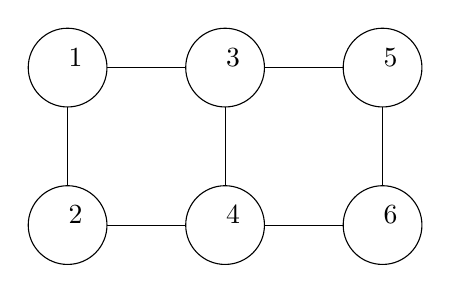
\begin{tikzpicture}
  %ノード1  
  \draw(4,2) circle (0.5)
  node[at={(4.1,2.1)}] {
    \begin{tabular}{c}
      1
    \end{tabular}
  };
  %ノード2  
  \draw(4,0) circle (0.5)
  node[at={(4.1,0.1)}] {
    \begin{tabular}{c}
      2
    \end{tabular}
  };
  %ノード3  
  \draw(6,2) circle (0.5)
  node[at={(6.1,2.1)}] {
    \begin{tabular}{c}
      3
    \end{tabular}
  };
  %ノード4  
  \draw(6,0) circle (0.5)
  node[at={(6.1,0.1)}] {
    \begin{tabular}{c}
      4
    \end{tabular}
  };
  %ノード5  
  \draw(8,2) circle (0.5)
  node[at={(8.1,2.1)}] {
    \begin{tabular}{c}
      5
    \end{tabular}
  };
  %ノード6  
  \draw(8,0) circle (0.5)
  node[at={(8.1,0.1)}] {
    \begin{tabular}{c}
      6
    \end{tabular}
  };
\draw(4,0.5) --(4,1.5);
\draw(6,0.5) --(6,1.5);
\draw(8,0.5) --(8,1.5);
\draw(4.5,0) --(5.5,0);
\draw(4.5,2) --(5.5,2);
\draw(6.5,0) --(7.5,0);
\draw(6.5,2) --(7.5,2);
\end{tikzpicture}

\caption{入力となる重み付き無向グラフの例}
\label{graphexample}
\end{center}
\end{figure}
%%%%%%%%%%%%%%%%%%%%%%%%%%%%%%

%%%%%%%%%%%%%%%%%%%%%%%%%%%%%%
\lstinputlisting[float=t,caption={%
図~\ref{graphexample}のASPファクト表現},%
captionpos=b,frame=single,label=code:graph_example.lp,%
numbers=none,%
breaklines=true,%
columns=fullflexible,keepspaces=true,%
basicstyle=\ttfamily\scriptsize]{code/graph_example.lp}
%%%%%%%%%%%%%%%%%%%%%%%%%%%%%%


本節では,最短ハミルトン閉路問題の例にとって,
入力となる重み付き無向グラフ(図~\ref{graphexample})の
ASP ファクト形式について説明する.
%
このグラフは,頂点数が6,辺の数が7であり,辺に付けられた値は距離を表す.
コード~\ref{code:graph_example.lp}に,ASPファクト形式を示す.
%
アトム\code{node/1}は頂点,\code{edge/2}は辺,\code{cost/3}は距離を表す.
例えば,\code{cost(1,2,3)}は,辺\code{edge(1,2)}の距離が3であることを
表している.

%%%%%%%%%%%%%%%%%%%%%%%%%%%%%%%%%%%%%%%%%%%%%%%%%%%%%%%%%%%%%%%%%%%%%%%
\section{ハミルトン閉路問題の ASP 符号化}\label{hamiltonianasp}
%%%%%%%%%%%%%%%%%%%%%%%%%%%%%%%%%%%%%%%%%%%%%%%%%%%%%%%%%%%%%%%%%%%%%%%

ハミルトン閉路問題は,与えられたグラフの全頂点をちょうど一度ずつ通る閉
路(ハミルトン閉路)が存在するかどうかを判定する問題である.
$G=(V,E)$にハミルトン閉路が存在する必要十分条件は,
以下の2つの制約を満たす部分グラフ$G'=(V,E')$が存在することである.

\begin{itemize}
\item $G'$の各頂点の次数が2 (次数制約)
\item $G'$が連結である (連結制約)
\end{itemize}

本論文では,前者を\textbf{次数制約},後者を\textbf{連結制約}と呼ぶ.
ハミルトン路問題は,ハミルトン閉路問題から始点と終点が一致するという閉
路の条件を取り除いたものである.
ハミルトン路問題では,次数制約は以下のように変わる.

\begin{itemize}
\item 始点と終点の次数が1,他の頂点の次数が2
\end{itemize}

以下では,ハミルトン閉路問題に対する3つの ASP 符号化
\textsf{undirected},\textsf{directed},\textsf{acyclicity}
を提案する.

%%%%%%%%%%%%%%%%%%%%%%%%%%%%%%%%%%%%%%%%%%%%%%%%%%%%%%%%%%%%%%%%%%%%%%%
\subsection{\textsf{undirected}符号化}
%%%%%%%%%%%%%%%%%%%%%%%%%%%%%%%%%%%%%%%%%%%%%%%%%%%%%%%%%%%%%%%%%%%%%%%

%%%%%%%%%%%%%%%%%%%%%%%%%%%%%%
\lstinputlisting[float=t,caption={%
\textsf{undirected}符号化},%
captionpos=b,frame=single,label=code:hamilton1.lp,%
numbers=left,%
breaklines=true,%
columns=fullflexible,keepspaces=true,%
basicstyle=\ttfamily\footnotesize]{code/hamilton1.lp}
%%%%%%%%%%%%%%%%%%%%%%%%%%%%%%

\textsf{undirected}符号化は,ハミルトン閉路問題の次数制約と連結制約を,
ASP の一貫性制約で表した基本的な符号化である.
コード~\ref{code:hamilton1.lp}に,\textsf{undirected}符号化を示す.
この符号化は,ハミルトン閉路問題とハミルトン路問題の両方に対応している.
符号化中の\code{s}は始点の頂点番号,\code{t}は終点の頂点番号を表し,こ
れらは実行時に与えられる.
ここでは,ハミルトン閉路問題(\code{s}=\code{t})の場合について説明する.

\begin{itemize}
\item 1行目のルールは,各辺\code{edge(X,Y)}に対して,その辺がハミルト
  ン閉路に含まれるかどうかを意味するアトム\code{in(X,Y)}を選択子を用い
  て導入している.
\item 次数制約は3行目のルールで表される.このルールは,
  各頂点\code{node(X)}に対して,その次数の和が2に等しいことを個数制約
  を使って表している.
\item 連結制約は11行目のルールで表される.
ある頂点\code{X}が始点\code{s}から到達可能であることを意味する補助アト
ム\code{reached(X)}を導入する.
8行目のルールは,始点\code{s}が到達可能あることを表している.
9行目のルールは,各辺\code{X}--\code{Y}に対して,その辺がハミルトン閉
路に含まれ(\code{in(X,Y)}),かつ,頂点\code{X}が始点から到
達可能であれば(\code{reached(X)}),\code{Y}も到達可能であることを表している.
10行目は9行目と同様であるが,辺\code{Y}--\code{X}の場合を表している.
11行目のルールは,各頂点\code{node(X)}が始点から到達可能でなければな
らないことを一貫性制約を使って表している.
\end{itemize}

%%%%%%%%%%%%%%%%%%%%%%%%%%%%%%%%%%%%%%%%%%%%%%%%%%%%%%%%%%%%%%%%%%%%%%%
\subsection{\textsf{directed}符号化}
%%%%%%%%%%%%%%%%%%%%%%%%%%%%%%%%%%%%%%%%%%%%%%%%%%%%%%%%%%%%%%%%%%%%%%%

%%%%%%%%%%%%%%%%%%%%%%%%%%%%%%
\lstinputlisting[float=t,caption={%
\textsf{directed}符号化},%
captionpos=b,frame=single,label=code:hamilton2.lp,%
numbers=left,%
breaklines=true,%
columns=fullflexible,keepspaces=true,%
basicstyle=\ttfamily\footnotesize]{code/hamilton2.lp}
%%%%%%%%%%%%%%%%%%%%%%%%%%%%%%

\textsf{directed}符号化は,\textsf{undirected}符号化をベースに,
与えられた無向グラフの各辺$u-v$に対して,2つの弧$u\rightarrow v$と
$v\rightarrow u$を対応させることで有向グラフ化して解く符号化である.
コード~\ref{code:hamilton2.lp}に,\textsf{directed}符号化を示す.
前節と同様に,ハミルトン閉路問題(\code{s}=\code{t})の場合について説明する.

\begin{itemize}
\item 1行目では,無向グラフの有向グラフ化を行う.
  与えられた無向グラフの各辺\code{edge(X,Y)}に対して,
  2つの弧\code{edge(X,Y)},\code{edge(Y,X)}を導入した.
\item 2行目のルールは,各弧\code{edge(X,Y)}に対して,その弧がハミルト
  ン閉路に含まれるかどうかを意味するアトム\code{in(X,Y)}を選択子を用い
  て導入している.
\item 次数制約は4,5行目のルールで表される.
  4行目では,各頂点\code{node(X)}に対して,
  その出次数が1に等しいことを個数制約を使って表している.
  5行目では,入次数について4行目と同様の制約を表す.
\item 連結制約は15行目のルールで表される.
  ある頂点\code{X}が始点\code{s}から到達可能であることを意味する
  補助アトム\code{reached(X)}を導入する.
  13行目のルールは,始点\code{s}が到達可能あることを表している.
  14行目のルールは,各弧\code{X}--\code{Y}に対して,その弧がハミルトン閉路
  に含まれ(\code{in(X,Y)}),かつ,頂点\code{X}が始点から
  到達可能であれば(\code{reached(X)}),\code{Y}も到達可能であることを表している.
  15行目のルールは,各頂点\code{node(X)}が始点から到達可能でなければ
  ならないことを一貫性制約を使って表している.
\item 18行目のルールは,解についての対称性を除去する.
  与えられた無向グラフ上の各ハミルトン閉路に対して,
  それを変換した有向グラフ上のハミルトン閉路は対称な2つが存在する.
  これによる解の重複を防ぐために,18行目のルールは,各弧\code{s}--\code{X},
  \code{Y}--\code{s}がハミルトン閉路に含まれるならば(\code{in(s,X),in(Y,s)}),
  \code{X < Y}でなければならないことを,一貫性制約を用いて表している
\end{itemize}

%%%%%%%%%%%%%%%%%%%%%%%%%%%%%%%%%%%%%%%%%%%%%%%%%%%%%%%%%%%%%%%%%%%%%%%
\subsection{\textsf{acyclicity}符号化}
%%%%%%%%%%%%%%%%%%%%%%%%%%%%%%%%%%%%%%%%%%%%%%%%%%%%%%%%%%%%%%%%%%%%%%%

%%%%%%%%%%%%%%%%%%%%%%%%%%%%%%
\lstinputlisting[float=t,caption={%
\textsf{acyclicity}符号化},%
captionpos=b,frame=single,label=code:hamilton3.lp,%
numbers=left,%
breaklines=true,%
columns=fullflexible,keepspaces=true,%
basicstyle=\ttfamily\footnotesize]{code/hamilton3.lp}
%%%%%%%%%%%%%%%%%%%%%%%%%%%%%%

\textsf{acyclicity}符号化は,\textsf{directed}符号化をベースに,
連結の制約に代わる部分閉路禁止制約を組込み非閉路制約で表現した符号化である.
コード~\ref{code:hamilton3.lp}に,\textsf{acyclicity}符号化を示す.
前節と同様に,ハミルトン閉路問題(\code{s}=\code{t})の場合について説明する.

\begin{itemize}
\item 1行目では,無向グラフの有向グラフ化を行う.
  与えられた無向グラフの各辺\code{edge(X,Y)}に対して,
  2つの弧\code{edge(X,Y)},\code{edge(Y,X)}を導入した.
\item 2行目のルールは,各弧\code{edge(X,Y)}に対して,その弧がハミルト
  ン閉路に含まれるかどうかを意味するアトム\code{in(X,Y)}を選択子を用い
  て導入している.
\item 次数制約は4,5行目のルールで表される.
  4行目では,各頂点\code{node(X)}に対して,
  その出次数が1に等しいことを個数制約を使って表している.
  5行目では,入次数について4行目と同様の制約を表す.
\item 部分閉路禁止制約は14行目のルールで表される.
  このルールは,始点でない各頂点\code{X},\code{Y}について,
  弧\code{X}--\code{Y}がハミルトン閉路に含まれるならば(\code{in(X,Y)}),
  そのような弧の集合をもつグラフが閉路をもたないことを,\code{#edge}宣言を用いて表す.
  ようするに,始点(終点)を含まないような閉路を禁止している.
\item 17行目のルールは,解についての対称性を除去する.
  与えられた無向グラフ上の各ハミルトン閉路に対して,
  それを変換した有向グラフ上のハミルトン閉路は対称な2つが存在する.
  これによる解の重複を防ぐために,17行目のルールは,各弧\code{s}--\code{X},
  \code{Y}--\code{s}がハミルトン閉路に含まれるならば(\code{in(s,X),in(Y,s)}),
  \code{X < Y}でなければならないことを,一貫性制約を用いて表している
\end{itemize}

%%%%%%%%%%%%%%%%%%%%%%%%%%%%%%%%%%%%%%%%%%%%%%%%%%%%%%%%%%%%%%%%%%%%%%% 
\section{最短ハミルトン閉路問題のASP符号化}\label{minexpl}
%%%%%%%%%%%%%%%%%%%%%%%%%%%%%%%%%%%%%%%%%%%%%%%%%%%%%%%%%%%%%%%%%%%%%%% 

%% %%%%%%%%%%%%%%%%%%%%%%%%%%%%%%
%% \lstinputlisting[caption =  最適化,label = minimize]{code/obj_minimize.lp}
%% %%%%%%%%%%%%%%%%%%%%%%%%%%%%%%

%%%%%%%%%%%%%%%%%%%%%%%%%%%%%%
\lstinputlisting[float=t,caption={%
最小化},%
captionpos=b,frame=single,label=code:obj_minimize.lp,%
numbers=left,%
breaklines=true,%
columns=fullflexible,keepspaces=true,%
basicstyle=\ttfamily\footnotesize]{code/obj_minimize.lp}
%%%%%%%%%%%%%%%%%%%%%%%%%%%%%%

最短ハミルトン閉路問題の目的関数は,
ハミルトン閉路を構成する各辺の距離の総和である.
コード\ref{code:obj_minimize.lp}は,
その目的関数の最小化を表す.
このコードは,各辺\code{edge(X,Y)}に対して,その辺がハミルトン閉路に
含まれ(\code{in(X,Y)}),その距離が\code{C}である時に(\code{cost(X,Y,C)}),
\code{C}の総和の最小化を,最小化関数を用いて表している.
.
%%%%%%%%%%%%%%%%%%%%%%%%%%%%%%
\lstinputlisting[float=t,caption={%
重み付き無向グラフの有向グラフ化},%
captionpos=b,frame=single,label=code:cost_both.lp,%
numbers=left,%
breaklines=true,%
columns=fullflexible,keepspaces=true,%
basicstyle=\ttfamily\footnotesize]{code/cost_both.lp}
%%%%%%%%%%%%%%%%%%%%%%%%%%%%%%

符号化directed,acyclicityについては,
与えられた無向グラフの各辺\code{edge(X,Y)}に対して,
2つの弧\code{edge(X,Y)},\code{edge(Y,X)}を導入した.
各辺の距離もこれに対応させるために,コード\ref{code:cost_both.lp}
を追加した.
このルールは,各辺\code{X}--\code{Y}の距離を表す\code{cost(X,Y,C)}について,
\code{cost(Y,X,C)}を導入する.
これにより,与えられた無向グラフの各辺\code{edge(X,Y)}の重み\code{C}が
2つの弧\code{edge(X,Y)},\code{edge(Y,X)}にも付与された.

%%%%%%%%%%%%%%%%%%%%%%%%%%%%%%%%%%%%%%%%%%%%%%%%%%%%%%%%%%%%%%%%%%%%%%% 
\section{コスト制約付きハミルトン閉路のASP符号化}
%%%%%%%%%%%%%%%%%%%%%%%%%%%%%%%%%%%%%%%%%%%%%%%%%%%%%%%%%%%%%%%%%%%%%%% 

%%%%%%%%%%%%%%%%%%%%%%%%%%%%%%
\lstinputlisting[float=t,caption={%
コスト制約},%
captionpos=b,frame=single,label=code:cost_constraint.lp,%
numbers=left,%
breaklines=true,%
columns=fullflexible,keepspaces=true,%
basicstyle=\ttfamily\footnotesize]{code/cost_constraint.lp}
%%%%%%%%%%%%%%%%%%%%%%%%%%%%%%

コスト制約付きハミルトン閉路問題は
ハミルトン閉路問題に,距離の総和が所与の閾値以下 (または以上) であること
を制約条件として付加した問題である.
コード\ref{code:const_constraing.lp}のルールは,その制約を表す.
ルール中の\code{c}は閾値を表し,これは実行時に与えられる.
このルールは,各辺\code{edge(X,Y)}に対して,その辺がハミルトン閉路に
含まれ(\code{in(X,Y)}),その距離が\code{C}である時に(\code{cost(X,Y,C)}),
\code{C}の総和が\code{c}以下でなければならないことを,
一貫性制約と重み付き個数制約を用いて表す.

また,\ref{minexpl}と同様に,
符号化directed,acyclicityについては,
アトム\code{cost}についても有向グラフ化に
対応させるためにコード\ref{code:cost_both.lp}を追加した.
%%%%%%%%%%%%%%%%%%%%%%%%%%%%%%%%%%%%%%%%%%%%%%%%%%%%%%%%%%%%%%%%%%%%%%%

%%% Local Variables:
%%% mode: latex
%%% TeX-master: "paper"
%%% End:

  \end{table}
\end{frame}

%%%%%%%%%%%%%%%%%%%%%%%%%%%%%%%%%%%%%%%%%%%%%%%%%%
%% ASPのコード
%%%%%%%%%%%%%%%%%%%%%%%%%%%%%%%%%%%%%%%%%%%%%%%%%%
\begin{frame}[fragile]{補足 : 根付き全域森 基本符号化}
%%%%%%%%%%%%%%%%%%%%%%%%%%%%%%%%% 
\lstinputlisting[frame=single,label=code:roop,%
xleftmargin=1zw,%
xrightmargin=1zw,%
numbersep=5pt,%
numbers=left,%
breaklines=true,%
columns=fullflexible,keepspaces=true,%
basicstyle=\ttfamily\scriptsize]{code/srf1.lp}
%%%%%%%%%%%%%%%%%%%%%%%%%%%%%%%%%
\end{frame}

\begin{frame}[fragile]{補足 : 遷移問題 シングルショット符号化}

\begin{multicols*}{2}
%%%%%%%%%%%%%%%%%%%%%%%%%%%%%%%%% 
\lstinputlisting[frame=single,label=code:roop,%
xleftmargin=1zw,%
xrightmargin=1zw,%
numbersep=5pt,%
numbers=left,%
breaklines=true,%
columns=fullflexible,keepspaces=true,%
basicstyle=\ttfamily\tiny]{code/trans-const.lp}
%%%%%%%%%%%%%%%%%%%%%%%%%%%%%%%%%
\end{multicols*}
\end{frame}

\begin{frame}[fragile]{補足 : 遷移問題 マルチショット符号化}
\begin{multicols*}{2}
%%%%%%%%%%%%%%%%%%%%%%%%%%%%%%%%%
\lstinputlisting[frame=single,label=code:incmode,% 
xleftmargin=1zw,%
xrightmargin=1zw,%
numbersep=5pt,%
numbers=left,%
breaklines=true,%
columns=fullflexible,keepspaces=true,%
basicstyle=\ttfamily\tiny]{code/dnet-trans.lp}
%%%%%%%%%%%%%%%%%%%%%%%%%%%%%%%%% 
\end{multicols*}
\end{frame}

\backupend

\end{document}

%%% Local Variables:
%%% mode: japanese-latex
%%% TeX-master: t
%%% End:
